\begin{savequote}[75mm]
The beginning is the most important part of the work.
\qauthor{Plato, The Republic}
\end{savequote}

% pending plagiarism check
\begin{flushleft}
\chapter{Image-based profiling identifies molecular determinants of cancer organoid architecture and plasticity}

\newpage

\section{Disclosure}
Significant parts of this chapter have been adapted from own manuscripts, including \textit{Image-based profiling identifies molecular determinants of cancer organoid architecture and plasticity} \cite{Betge2019MultiparametricOrganoids} and its public pre-print versions. The maximum contrast projection method, organoid segmentation method, feature extraction procedure and organoid viability classification (LDC) was previously developed by Jan Sauer as part of his dissertation. Image-based profiling experiments were supported by Johannes Betge and Clara Dingert. 

\section{Establishing patient derived organoids for image-based profiling}

Patient derived organoids can be established from diverse healthy or malignant tissues and have been shown to represent their tissue of origin with respect to morphological and molecular features including gene expression and somatic mutations \cite{Fujii:2016jo, Weeber2015-sn, Van_De_Wetering2015-ko, Sato:2011-1h,  Broutier2017-wg}. To generate personalized cancer models for image-based profiling, I designed and implemented a standardized laboratory workflow to generate patient derived organoids from colorectal cancer samples via endoscopic biopsy (Figure 1a). Briefly, fresh patient samples were washed, digested and embedded in a basal membrane extract, a proprietary mixture of extracellular matrix proteins especially rich in Laminin and Collagen 4. The isolated tumor cells were then overlaid with a growth factor rich medium, containing Epidermal Growth Factor (EGF), the BMP-signaling antagonist Noggin and the small-molecule inhibitor A83-01, which inhibits TGF\beta-signaling by targeting the Activin receptor-like kinase family.

%\clearpage
\begin{figure}[h]
\centering
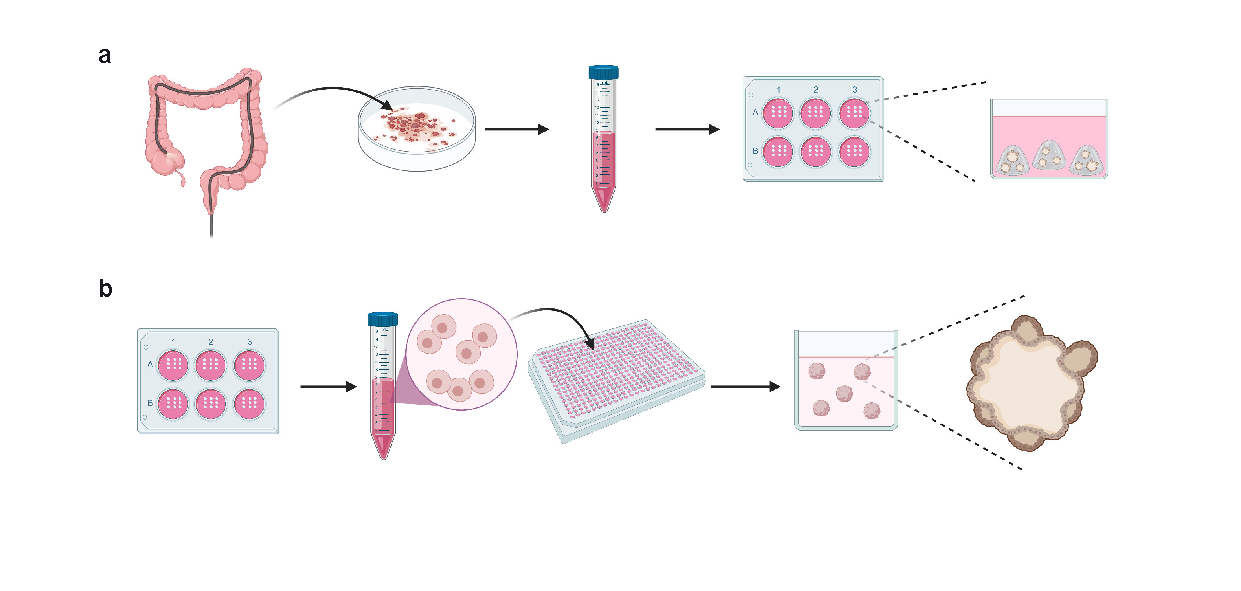
\includegraphics[width=\textwidth,
                height=\textheight,
                keepaspectratio]{figures/pdf/fig_110.pdf}
\caption{\textbf{Central liquid handling methods a} Organoid isolation procedure. Colorectal cancer tissue biopsies were collected via endoscopy, enzymatically removed from extracellular matrix proteins, washed and resuspended in basal membrane extract hydrogel. After solidification of hydrogel domes, organoids were overlayed with growth factor rich culture medium. \textbf{b} Organoid high-throughput experimentation. Colorectal cancer organoids were harvested, partially digested, seeded in hydrogel-coated 384-well plates}
\label{fig_110}
\end{figure}

Following this protocol, patient derived organoids from 13 patients with colorectal cancer were prospectively developed. Donors to the biobank represented different UICC stages (Figure \ref{S1_mod}). Gene expression profiling and amplicon sequencing of frequently altered genes in colorectal cancer showed molecular profiles characteristic for the disease . Similar to sequencing studies of primary tumors, patient derived organoids harbored a high frequency of APC (6/13), KRAS (8/13) and TP53 (5/13) mutations \cite{Muzny2012-hr}. On a gene expression level, patient derived organoids mainly represented the canonical consensus molecular subtype CMS 2 of colorectal cancer \cite{Guinney2015-ex}. No patient derived organoid line with a MSI-high phenotype and the associated CMS 1 molecular subtype was established. Also, no organoid line matched the molecular subtype CMS 4, which is associated with stromal infiltration and TGF\(\beta\)-signaling. These results are in line with previous observations \cite{Van_De_Wetering2015-ko, Schutte2017-fl} and the limitations of the organoid culture system, which selects for growth of epithelial cells (favored by canonical Wnt signaling high, BMP4 signaling low) over mesenchymal cells (favored by canonical Wnt signaling low, BMP4 signaling high) \textit{ex vivo} \cite{Sato2011-lh}.

\clearpage
\begin{figure}[h]
\centering
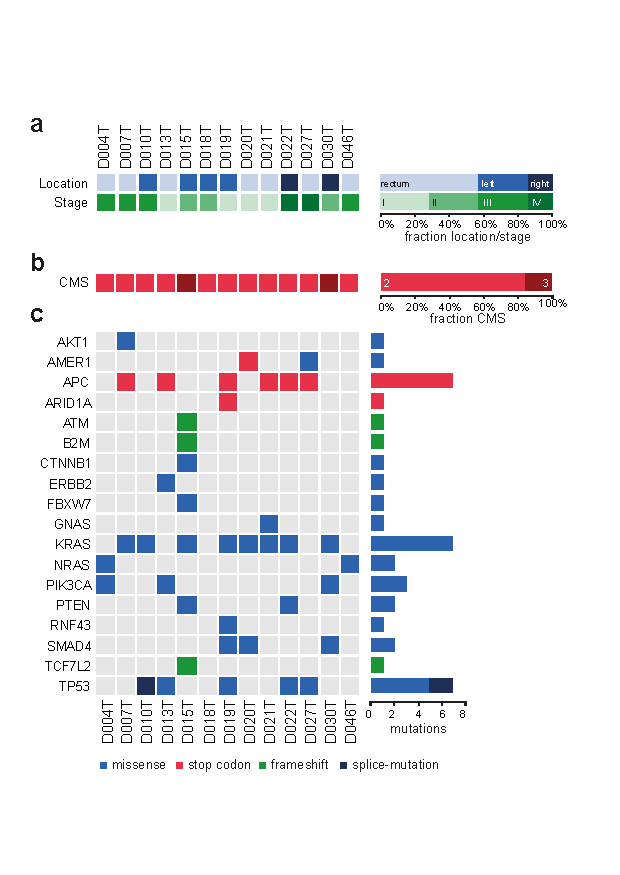
\includegraphics[width=\textwidth,
                height=\textheight,
                keepaspectratio]{figures/pdf/fig_120.pdf}
\caption{\textbf{Organoid cohort overview a} Tumor location (right/left/rectum) and AJCC/UICC stage of colorectal cancers that patient derived organoids were derived from. \textbf{b}  Consensus molecular subtypes of organoids determined by RNA expression analysis. \textbf{c} Mutation status in PDOs, as analyzed by amplicon sequencing. Figure created with support from Johannes Betge (graphical presentation),  Erica Valentini (sequencing data analysis) and Benedikt Rauscher (CMS type inference)}
\label{fig_120}
\end{figure}
\clearpage


\section{Enabling methods for high-throughput image-based profiling of organoids}
To systematically measure organoid morphology, I established a platform for high-throughput image-based profiling experiments. The three engineering problems that had to be solved were (1) control of organoid size and density in a 384-well plate format, (2) control of organoid location within the hydrogel for efficient microscopy and (3) maintenance of organoid integrity during automatic fixation and permeabilization. 

\begin{figure}[h]
\centering
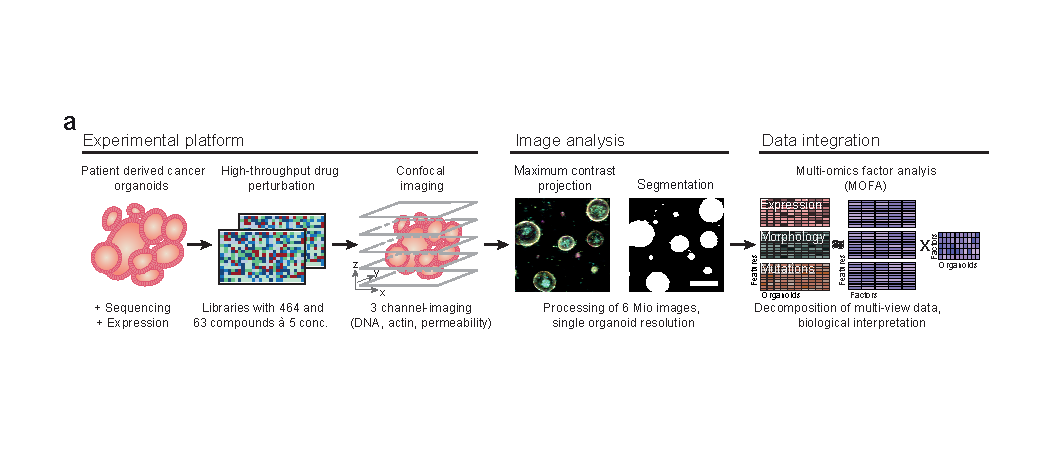
\includegraphics[width=\textwidth,
                height=\textheight,
                keepaspectratio]{figures/pdf/fig_130.pdf}
\caption{\textbf{Overview of experiments a} Organoids were isolated from endoscopic biopsies from patients with colorectal cancer. Organoids were dissociated and evenly seeded in 384-well plates before perturbation with an experimental (464 compounds) and a clinical compound library (63 compounds à 5 concentrations, 842 perturbations across both libraries). After treatment, high-throughput fluorescence microscopy was used to capture the morphology of organoids.  The multi-channel (DNA, beta-actin, cell permeability) 3D imaging data was projected, segmented, and descriptive features were extracted to quantify potential drug-induced phenotypes. Untreated organoid morphology, organoid size and drug activity scores were integrated with mRNA expression and mutation data in a Multi-Omics Factor Analysis (MOFA) to increase interpretability of organoid variation. Figure created with support from Johannes Betge (graphical presentation)}
\label{fig_130}
\end{figure}

\bigbreak

A standard protocol for cell-based assays, including image-based profiling, is seeding cells into microwell plates at a fixed cell number. In order to determine cell number, adherent cells are dissociated and counted using optical methods. Patient derived organoids, however, demonstrated a low rate of organoid outgrowth when passaged by complete organoid dissociation down to the single cell level. To improve organoid outgrowth, the dissociation protocol was stopped early, yielding cell clusters of ca. 1-10 cells. These organoid fragments showed an increased outgrowth rate, which could be further improved by treating cells with 10 μM of Rho-Kinase inhibitor Y-27632 (data not shown). To control organoid size and density, organoids were digested with a modified trypsin derivative, and filtered through a 40 um cell strainer to ensure an upper limit of organoid fragment size. To effectively estimate the cell number while maintaining organoid fragments, organoid fragments were titrated based on their ATP concentration, instead of cell count. The ATP concentration of the organoid fragment suspension was determined using an ATP-dependent luminescence readout. After controlling for ATP concentration, the organoid fragment suspension was seeded onto basal membrane extract covered 384 well plates.

\begin{figure}[h]
\centering
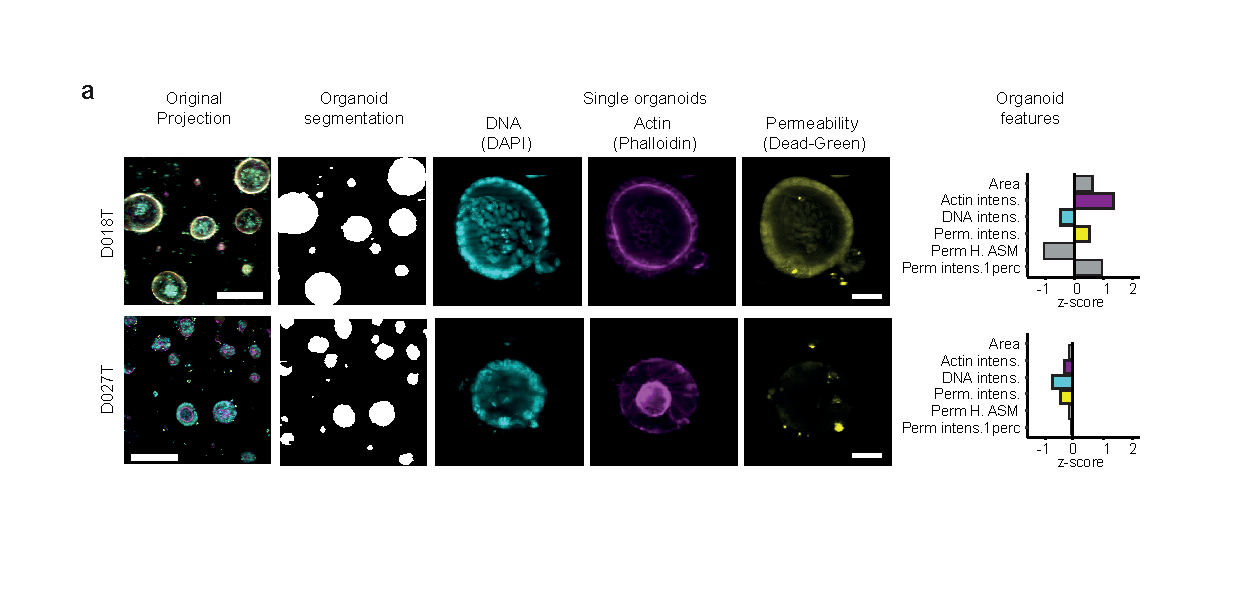
\includegraphics[width=\textwidth,
                height=\textheight,
                keepaspectratio]{figures/pdf/fig_135.pdf}
\caption{\textbf{Image-based profiling method a} The image-processing pipeline illustrated with representative example images from 2 organoid lines: Organoids were imaged at multiple layers along the z-axis. Images were projected using a maximum contrast projection and segmented using a convolutional neural network, both designed and implemented by Jan Sauer. Descriptive features were extracted from all three channels to quantify phenotypes. Feature plots show the median phenotype of unperturbed organoids, six example features (Area, Phalloidin intensity, DAPI intensity, FITC intensity, FITC Haralic angular second moment (ASM) and FITC intensity 1-percentile) and their z-scores relative to all profiled organoid lines are shown. Figure created with support from Jan Sauer (data processing) and Johannes Betge (graphical presentation)}
\label{fig_135}
\end{figure}

\bigbreak

Conventional image-based profiling of adherent cells is based on automatic microscopy of one 2D plane per field of view. Given the 3D growth patterns of organoids, more data has to be acquired to fully capture organoid phenotype. Acquiring multiple planes of imaging data per field of view, however, creates a technical data storage and processing burden. For a fixed 3D volume, the dimensions of the collected data increase linearly with the number of acquired planes and quadratically with the target z-axis resolution. To reduce the observed 3D volume and thus the number of required imaging planes, the vertical distribution of organoid fragments within the basal membrane extract layer was controlled by centrifuging organoid fragments post-seeding at 500G for 20 minutes at 37 degrees Celsius. The centrifugal force led to an accelerated sedimentation of organoid fragments onto the same optical plane before the polymerization of the hydrogel was complete.

\bigbreak

After three days of culture and four days of compound treatment, organoids were fixed and stained for actin (Phalloidin/TRITC), DNA (DAPI), and cell permeability (DeadGreen/FITC). Subsequently, plates were imaged at multiple z-positions by automated confocal microscopy. During treatment with the hyperosmolar fixative (3\% para-formaldehyde in phosphate buffered saline) the protein rich hydrogel underwent an irreversible volume contraction (data not shown). To reduce this artefact, the fixative was supplemented with bovine serum albumin to a final concentration of 1\% weight/volume. After image acquisition, 3D data was projected into a 2D plane by applying a maximum contrast projection followed by segmentation with a weakly-supervised convolutional neural network and single-organoid-level feature extraction \ref{fig_135}. In summary, seeding well-quantifiable organoid fragments instead of single cells, centrifuging organoid fragments to reduce the imaged 3D volume, and modifying liquid handling buffers to avoid hydrogel-driven artefacts technically enabled high-throughput image-based profiling of organoid models. 


\section{Image-based profiling captures the morphological diversity of patient-derived cancer organoids}

To better understand the diversity of organoid phenotypes and how morphology links to molecular processes, I performed image-based profiling at single organoid resolution with 11 organoid models using compounds targeting developmental pathways (464 compounds), as well as compounds in clinical use (63 compounds in 5 concentrations) \ref{fig_137}. The resulting data comprised morphological profiles for each organoid with 528 phenotypic features  that were subsequently reduced into 25 principle components representing 81\% of morphological variance.

\begin{figure}[h]
\centering
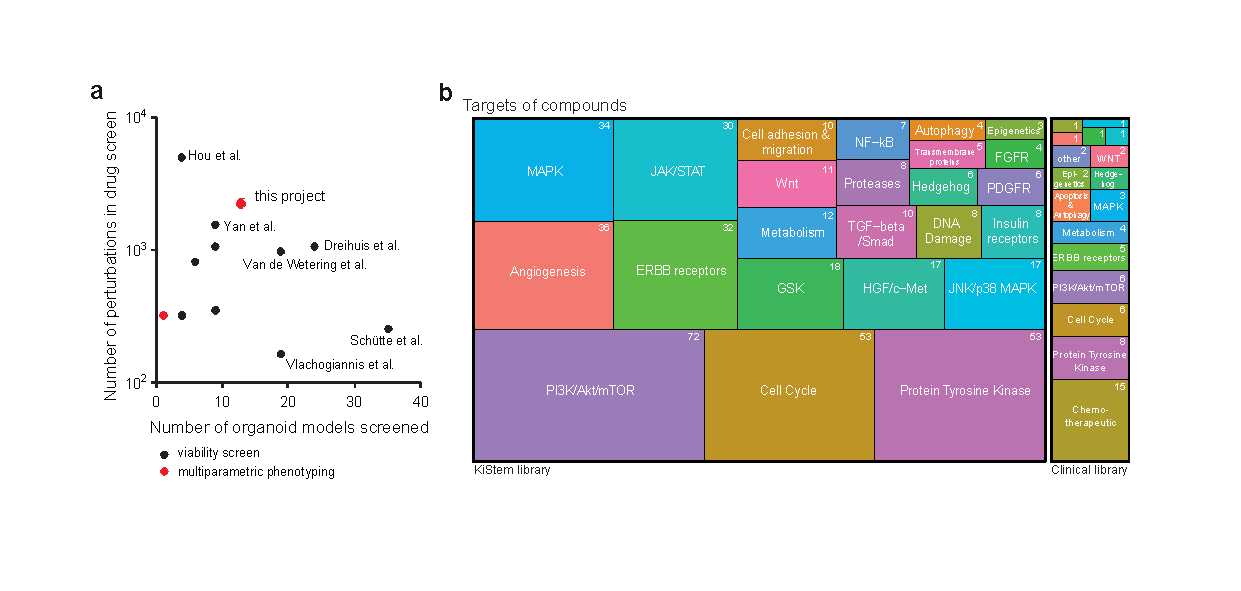
\includegraphics[width=\textwidth,
                height=\textheight,
                keepaspectratio]{figures/pdf/fig_137.pdf}
\caption{\textbf{Dataset dimensions and compound library overview a} Number of organoid models and number of perturbations in previous publications reporting high-throughput drug screenings with patient derived cancer organoids, \textbf{b} Graphical representation of the compound libraries used for drug screening in this project: A library targeting kinases and stem cell pathways (KiStem library, 464 compounds) and a clinical library with 63 drugs in 5 concentrations. Figure created with support from Johannes Betge (graphical presentation)}
\label{fig_137}
\end{figure}

\bigbreak

To visualize the heterogeneity of colorectal cancer organoids and drug induced changes across and within cancer organoid lines, the features of ca. 5.5 million profiled organoids were embedded using uniform manifold approximation and projection (UMAP) (figure \ref{fig_140} a and \ref{fig_145} a-c). Most organoid lines showed characteristic bimodal log-normal distributions of organoid size with one component containing small organoids and another component made up of larger organoids with varying, line specific, average size (figure \ref{fig_140} b, and \ref{fig_145} d-e). The log-normal-like size distribution likely resulted from intrinsic differences in cellular size and growth rate compounding over time in multicellular organoids. While DNA and actin staining intensity were positively correlated with organoid size, cell permeability was negatively correlated and enriched in regions with relatively smaller organoids (\ref{fig_145} a-c). Graph-based clustering of this identified 12 regions within the embedding (figure \ref{fig_140} c). When comparing drug-treated organoids to organoids treated with the negative control (DMSO), no clear separation of these two groups, except an increased presence of drug-treated organoids in region 3,  was seen. This finding suggested that organoid morphology was distributed on a continuum of phenotypes spanning perturbed and unperturbed conditions of the experiment (figure \ref{fig_145} f). 

\clearpage

\begin{figure}[h]
\centering
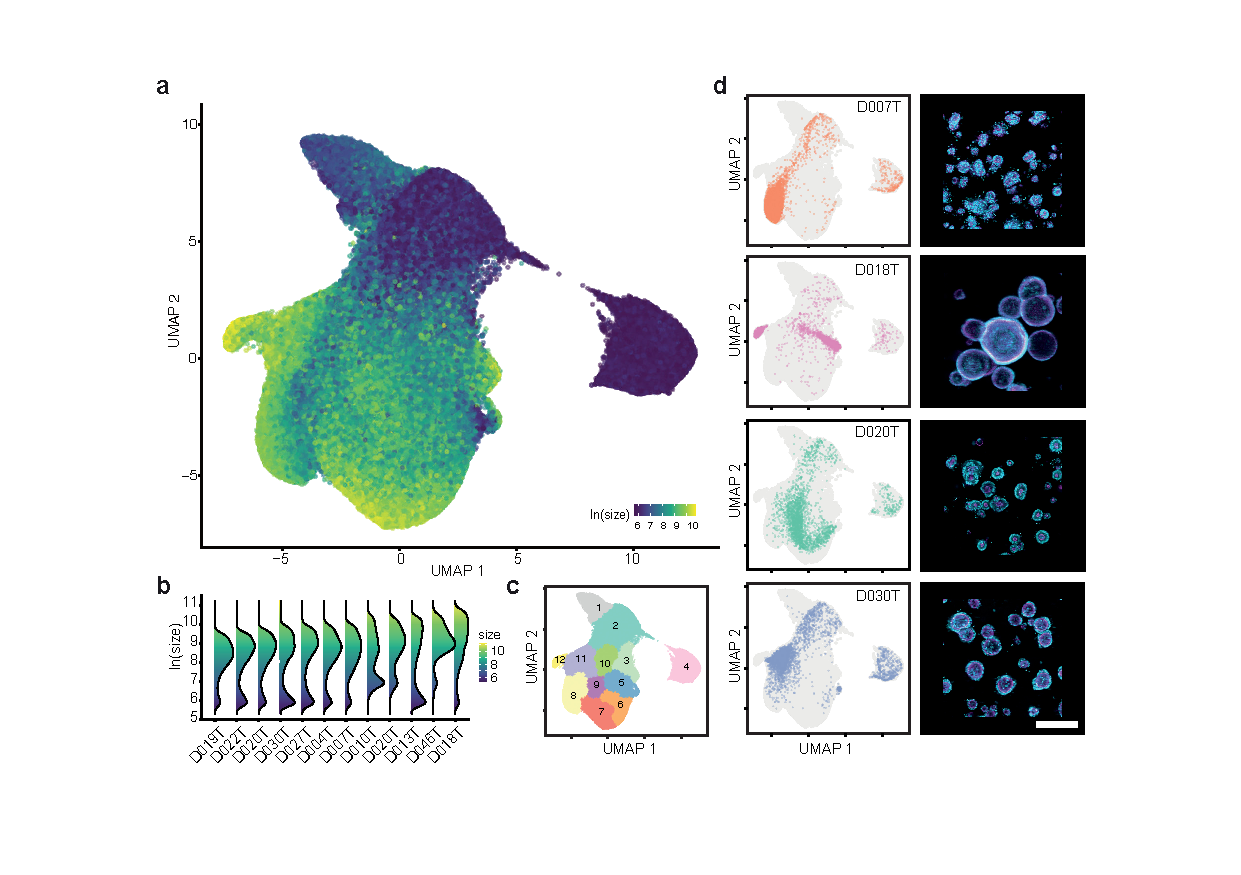
\includegraphics[width=\textwidth,
                height=\textheight,
                keepaspectratio]{figures/pdf/fig_140.pdf}
\caption{\textbf{Image-based profiling captures the phenotype diversity of patient derived cancer organoids a} Uniform Manifold Approximation and Projection (UMAP) of organoid-level features for a random 5\% sample out of ca. 5.5 million organoids. The same sample is used for visualizations throughout the figure. Color corresponds to the log-scaled organoid area (dark blue: minimum size, yellow: maximum size). \textbf{b} organoid size distribution across lines. \textbf{c} UMAP representation of DMSO treated and drug treated organoids. Graph-based clustering of organoids by morphology. \textbf{d} UMAP embeddings of selected organoid lines (baseline state / 0.1\% DMSO control-treated organoids) representing different morphological subsets, grey background consists of randomly sampled points. Depicted are representative example images for each line (right, cyan = DNA, magenta = actin, scale-bar: 200µm).}
\label{fig_140}
\end{figure}
\bigbreak

Different organoid lines within the embedding were located in characteristic regions, with organoid size and organoid architecture as primary organizing factors (figure \ref{fig_140} b and d). For example, organoid line D018T had the largest median organoid size within the dataset and a cystic organoid architecture, while D020T organoids had a solid architecture and smaller median size. In most cases, organoid lines had two areas of main density, with one of them in regions 2, 3 or 4, reflecting the previously mentioned bimodal size distribution. In summary, image-based profiling of patient derived colorectal cancer organoids showed strong morphological heterogeneity with line dependent differences in size and organoid architecture.

\begin{figure}[h]
\centering
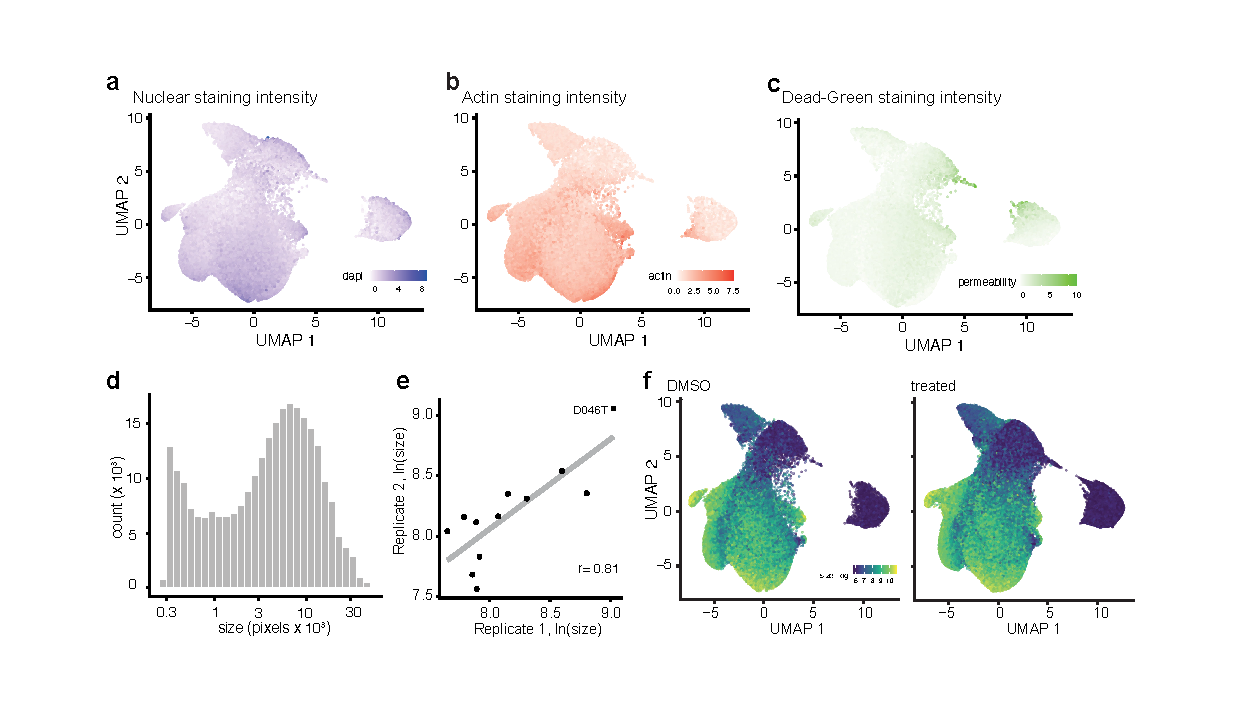
\includegraphics[width=\textwidth,
                height=\textheight,
                keepaspectratio]{figures/pdf/fig_145.pdf}
\caption{\textbf{Basic image-based features and their role in organoid phenotype diversity. a-c} Uniform Manifold Approximation and Projection (UMAP) of organoid-level features marked by DNA (DAPI) staining intensity (b), actin (Phalloidi/FITC) staining intensity (c) and permeability (DeadGreen) staining intensity \textbf{d} Distribution of organoid size for all control (DMSO) treated organoids. \textbf{e} Replicate correlation of organoid size for control treated organoids. \textbf{f} UMAP representation of DMSO treated and drug treated organoids}
\label{fig_145}
\end{figure}
\bigbreak

Exploratory data analysis of the relationship between organoid morphology and batch showed overall reproducible measurements of organoid profiles across experiments. While objects with a log-area of 8 pixels and larger showed reproducible phenotypes across contexts, smaller objects (mostly dead organoids) showed batch-dependent differences in phenotype. For example, region 1 within the UMAP embedding was exclusively occupied by observations from batch HC1092-09 and HC1092-10, while region 4 was relatively underoccupied. Given the confounding of line differences by experimental batches (experimental batches and tested organoid lines were not independent) and the stronger prevalence of batch effects for small objects, no procedure to remove these batch-dependent differences in organoid phenotype were performed. 

\bigbreak

\begin{figure}[h]
\centering
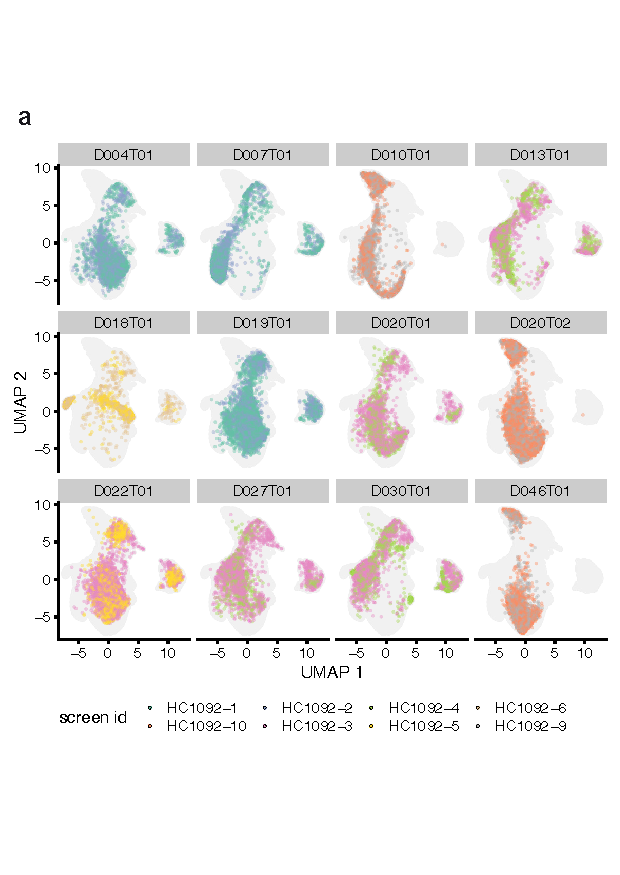
\includegraphics[width=\textwidth,
                height=\textheight,
                keepaspectratio]{figures/pdf/fig_150.pdf}
\caption{\textbf{Technical confounders and their impact on organoid phenotype. a} UMAP of organoid level features stratified by organoid line and colored by experimental batch.}
\label{fig_150}
\end{figure}
\clearpage


\section{Organoid phenotype-profiles capture organoid viability}

Drug induced changes in cell viability are a basic readout in oncology drug discovery. Prompted by the observation that organoid size was a major factor determining the structure of the phenotype embedding (UMAP and factor 1 in MOFA analysis, see below), I hypothesized that low organoid size was at least partially the result of cell death within the organoid and, more broadly, that phenotype data could be used to estimate organoid viability. Bortezomib, a small molecule proteasome inhibitor with high in vitro toxicity led to dose dependent organoid death in all organoid lines, thus representing suitable positive controls (Fig. 2a). Analogous to pseudotime in single-cell  gene expression analysis, we fitted dose-dependent trajectories of bortezomib (Fig. 2b) using a non-parametric principle curve fit. Starting from diverse baseline morphologies, increasing doses of this compound led to a step-wise convergence on a final death-related phenotype, which corresponded to the areas with enrichment of small objects (regions 2, 3 and 4). 

\begin{figure}[h]
\centering
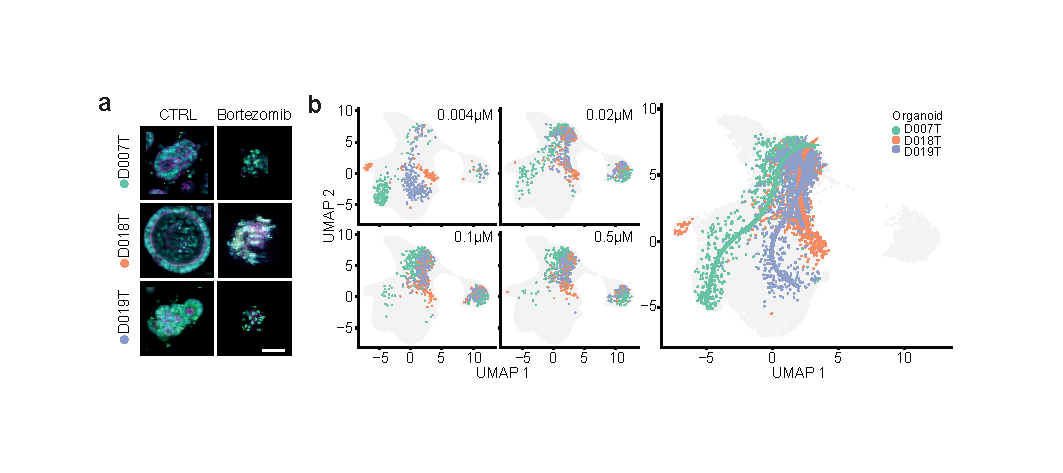
\includegraphics[width=\textwidth,
                height=\textheight,
                keepaspectratio]{figures/pdf/fig_160.pdf}
\caption{\textbf{Organoid phenotype-profiles capture organoid viability. a} Representative example images of negative- (0.1\% DMSO) and positive control treated organoids (2.5µM bortezomib, cyan = DNA, magenta = actin, yellow = cell permeability; average images were selected and embedded in black background; scale bar: 50µm). b, Dose-dependent-trajectory of bortezomib drug effect. UMAP of organoid morphology at different bortezomib doses and (right panel) dose-dependent trajectory for three representative organoid lines. For visual purposes, trajectory inference was limited to partition 1, the left-hand set of measurements within the UMAP, representing ca. 95 \% of all imaging data.}
\label{fig_160}
\end{figure}
\bigbreak

Similarly, paclitaxel, a microtubule disassembly inhibitor, shifted the bimodal size distribution of organoids in a dose-dependent fashion (figure \ref{fig_161}a), while organoid count remained largely unchanged (figure \ref{fig_161}b). This effect, however, was organoid line-specific, as median organoid size in paclitaxel sensitive lines (e.g. D022T) decreased, while the size of other organoids remained unaffected (e.g. D046T, Fig. 2c-f). These observations suggested a link between organoid morphology, especially organoid size, with a loss of cell viability. To further test the link between organoid morphology and cell viability, I performed a luminescence-based, ATP dependent, cell viability assay (CTG) in parallel with imaging as benchmark. A strong association of CTG viability with organoid size (Fig. 2g) was visible. 


\begin{figure}[h]
\centering
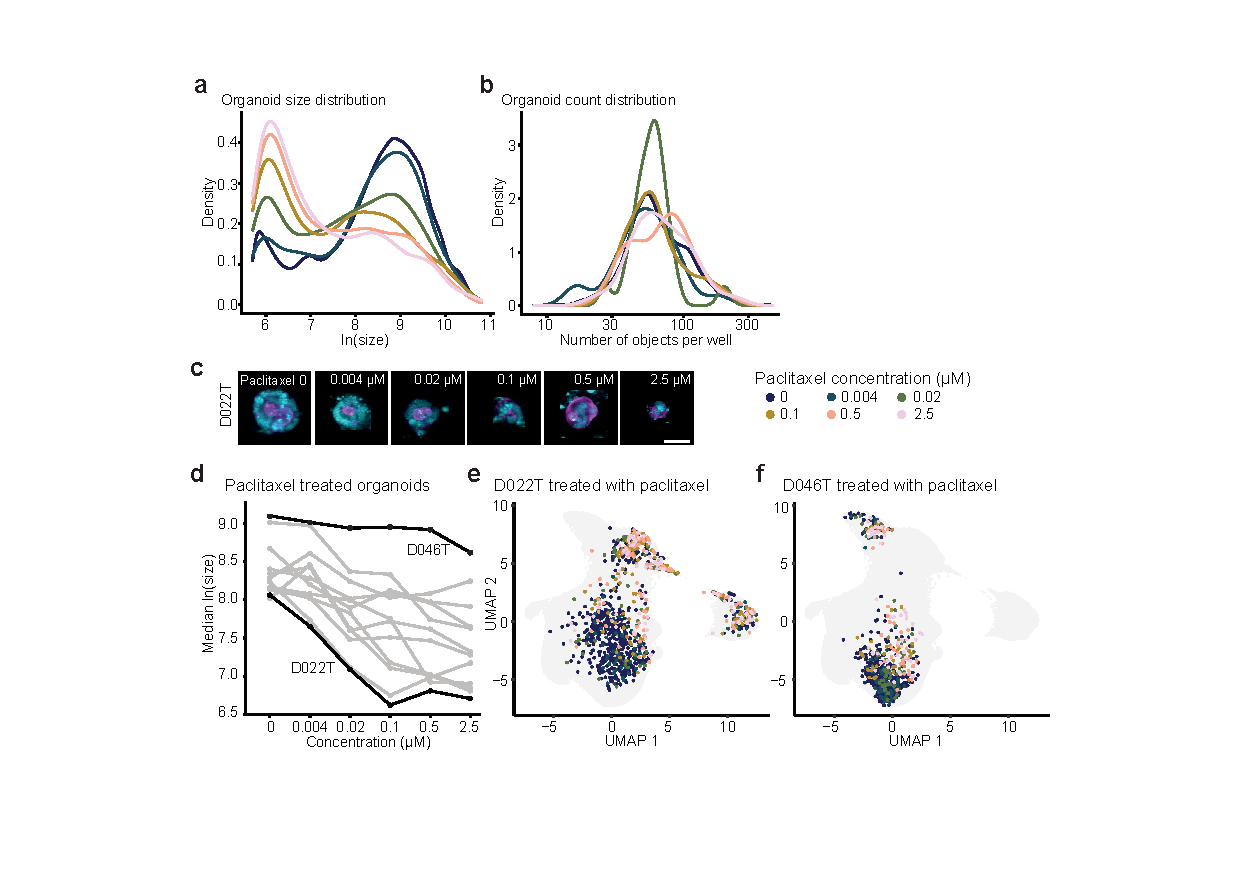
\includegraphics[width=\textwidth,
                height=\textheight,
                keepaspectratio]{figures/pdf/fig_161.pdf}
\caption{\textbf{Organoid phenotype-profiles capture treatment specific changes in organoid viability. a} Distribution of organoid size at different concentrations of paclitaxel. Shown is a random sample of 30\% of all paclitaxel treated organoids for this and following figures. \textbf{b} Distribution of organoid number per well at different concentrations of paclitaxel. \textbf{c} Example images of D022T organoids treated with paclitaxel. \textbf{d} Dose-response relationship of organoid size and paclitaxel dose. D022T and D046T are highlighted. \textbf{e} UMAP of organoid morphology highlighting D022T organoids treated at different concentrations of paclitaxel. \textbf{f} UMAP of organoid morphology highlighting D046T organoids treated at different concentrations of paclitaxel.}
\label{fig_161}
\end{figure}
\bigbreak

To test whether a more accurate prediction of organoid viability was achievable by using all available imaging data, I used a previously trained set of random forest classifiers (live/dead classifiers, LDC). These classifiers were trained on individual organoid phenotype profiles to distinguish between negative and positive control treatments (DMSO, bortezomib and sn-38, Supplemental Fig. S3d-e). When applying the classifier to the whole imaging dataset and visualizing predictions via UMAP, organoids within previously identified regions 2, 3 and 4 had the highest probabilities for death (Fig. 2h). LDC had the highest correlation with CTG based viability data (Fig. 2i), however, the association with organoid size was almost as strong in the majority of organoid lines (Fig. 2i, Supplemental Fig. S3g), while other simple features, such as DAPI actin, and permeability (DeadGreen) intensity were less suitable to predict viability of organoids (Fig 2i). In conclusion, organoid size is an informative metric to describe organoid viability, but is biased by line-specific differences in untreated organoid size. Models consuming more comprehensive morphological information can achieve even higher predictive performance of organoid viability. 

\begin{figure}[h]
\centering
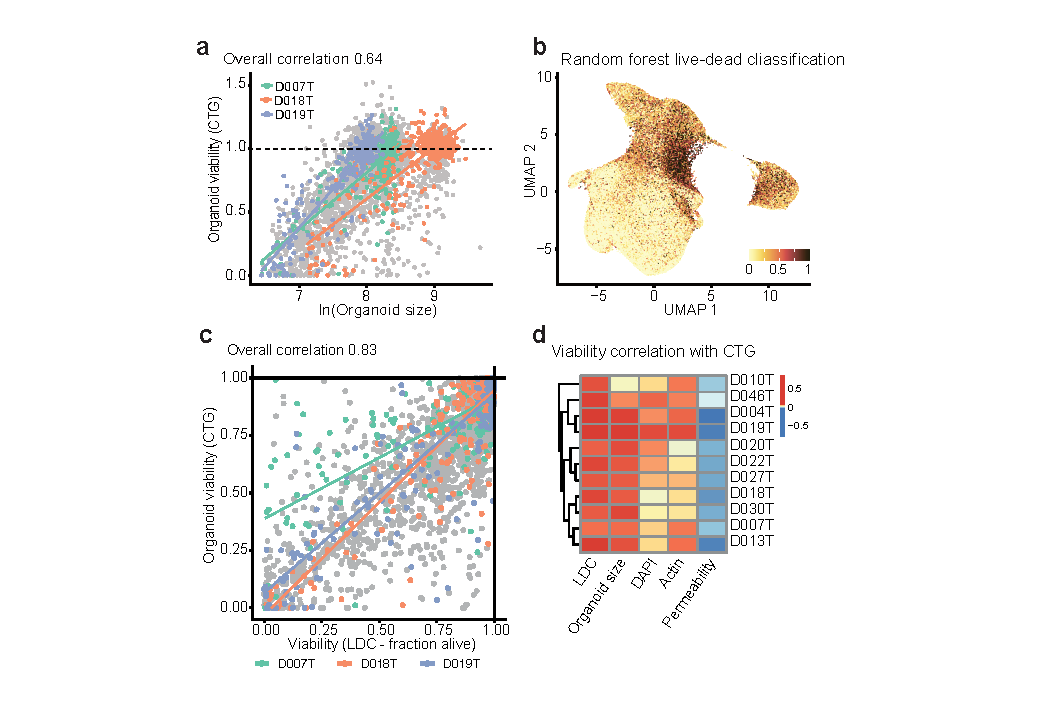
\includegraphics[width=\textwidth,
                height=\textheight,
                keepaspectratio]{figures/pdf/fig_162.pdf}
\caption{\textbf{Organoid phenotype-profiles reflect ATP-dependent viability measurements. a} Association of organoid size of selected example lines with organoid viability determined by luminescence-based, ATP-dependent viability profiling with CellTiter-Glo (CTG), which was performed in parallel with imaging on a subset of drug treatments. \textbf{b} UMAP visualization of dead organoids within our dataset, based on supervised machine learning of organoid viability using classifiers trained on positive- (high-dose bortezomib and SN-38) and negative (DMSO) controls (live-dead classifiers, LDC). \textbf{c} Association of organoid size of selected example lines with organoid viability determined by luminescence-based, ATP-dependent viability profiling with CellTiter-Glo (CTG), which was performed in parallel with imaging on a subset of drug treatments for benchmarking. \textbf{d} UMAP visualization of dead organoids within our dataset, based on supervised machine learning of organoid viability using classifiers trained on positive- (high-dose bortezomib and SN-38) and negative (DMSO) controls (live-dead classifiers, LDC). \textbf{e} Association of LDC and example organoid features (size, DAPI, actin and permeability dye intensities) with benchmark CTG viability read out. Figure created with support from Jan Sauer (LDC classifier training)}
\label{fig_162}
\end{figure}
\bigbreak

\section{Drug induced organoid phenotypes correspond to drug mechanism of action}

An advantage of image-based phenotyping over cell viability measurements in drug discovery is the ability to use the high dimensional drug-induced phenotype-profiles to identify active but not necessarily lethal drugs and estimate their mechanism of action by unsupervised clustering. To test whether this approach could be used in cancer organoids, we used a weakly supervised learning approach to identify drug effect vectors and group them by similarity. First, we trained logistic regression models to separate individual compound-treated organoids from unperturbed controls and used the resulting normal vector between control- and treated organoid profiles as the drug effect vector. Next we scored every model’s ability to separate treated and untreated organoids (AUROC, ranging from 0.5 to 1) to identify active treatments that induce a robust change in organoid morphology (Fig. 3a, 3b). Based on our observations, drug activity was necessary but not sufficient for a viability effect (Fig. 3c). A fraction of drugs led to identifiable changes in organoid morphology but were not classified as lethal by our LDC model. 
To test whether active drugs systematically induce organoid phenotypes that are informative of mechanism of action, we calculated the cosine distance between concatenated drug effect vectors. We identified a clustering of specific mode-of-actions, including inhibitors of MEK, Aurora kinase, CDK, mTOR, AKT, EGFR or GSK3 which we also identified with an alternative computational approach, phenotype profile averaging followed by pearson correlation (Fig. 3d-h, Supplemental Fig. S4a-c, S5a-c). Furthermore, compounds with related targets also induced similar phenotypes, for example MEK inhibitors clustered with specific RAF- and ERK inhibitors (Fig. 3e) or AKT and PI3K inhibitors were part of a cluster mainly containing mTOR targeting compounds (Fig. 3f, Supplemental Fig. 5a). The clustering also suggested additional mode-of-actions or off-target effects for well-described compounds (Fig. 3g-h). For example, the PKC inhibitor enzastaurin was related to GSK3, substantiating a previously described interaction with the alpha and beta subunits of GSK328 (Fig. 3h). To assess whether morphological profiles of active drug treatments were primarily driven by differences in organoid viability, we compared LDC predictions with the phenotypic clustering (Fig. 3i). We observed a larger cluster of lethal treatments (including molecules targeting ATM, JAK, PLK, CDK). However, the majority of clusters were caused by non-lethal phenotypes, including those induced by inhibitors of AKT, mTOR, EGFR or GSK3. Visual inspection of several phenotypes (Fig. 3j) revealed recurring drug target dependent phenotypes. Most notably, MEK inhibitors led to reorganization towards more cystic organoid architecture. These drug target dependent phenotypes were observable across organoid lines and drugs.

\section{Multi-omics factor analysis identifies shared factors linking morphology, genomic data and drug activity}

A limitation of image-based profiling experiments is that both unperturbed and drug induced phenotypes are challenging to interpret in terms of their underlying biology. Theoretically, in the presence of multiple in vitro models with both phenotype and genomic measurements, links between the two data modalities can be learned. Based on the observation that organoid morphology was distributed in a continuous space, we hypothesized that variation in organoid baseline morphology could be associated with differences in gene expression, mutations, as well as drug activity for the 11 cancer organoid lines in our sample. To learn a joint representation of unperturbed organoid morphology, unperturbed organoid size, gene expression, somatic mutations, and drug activity, we performed multi-omics factor analysis (MOFA).29 MOFA is a matrix factorization method that decomposes a set of different measurements into a shared table of factors scoring each observed sample and a set of corresponding tables linking each factor to features in the set of original measurements.29 When trained with a low number of k = 3 factors, MOFA recovered factors explaining ca. 41-24% of variance across the different data modalities, with the first two factors accounting for ca. 29-17% in aggregate (Supplemental Fig S6a-b). While gene expression, mutations and drug activity profiles for organoid lines contributed to all factors, factor 1 captured an exceptional amount of variation in median organoid size (ca. 39%). In contrast, factor 2 was primarily capturing variation within baseline organoid morphology (ca. 16%) (Fig 4a). Overall, MOFA factors explained up to 40% of variance in median organoid size, drug activity and gene expression, while less than 30% of variance in baseline organoid morphology was explained by the model (Fig 4b). Organoid lines D046T and D004T stood out as lines with the strongest score for factor 1, while lines D018T and D013T had the strongest score in factor 2. Visual inspection of organoids revealed that organoid lines with a higher factor 1 score tended to be larger in size and organoids with high factor 2 score tended to have a more cystic organoid architecture based on manual classification. We could not identify interpretable morphological differences between factor 3 low and high organoids and focused our subsequent analysis on the first two interpretable factors generated by MOFA (Supplemental Figures S6c). Overlaying untreated single organoid profiles with factor scores of their corresponding organoid line showed that regions within the embedding were characteristic for different factors (Fig 4d). Factor 1 high lines were located mostly in region 7 (the bottom part of the embedding) while factor 2 and 3 positive lines were located in region 3, 10, 11, 12 (the middle part of the embedding) and region 9 (a central part of the embedding), respectively. To summarize, MOFA identified factors within the dataset that explained variation between organoid lines across different data modalities, including organoid morphology and median size. 

\section{An LGR5+ stemness program is associated with cystic organoid architecture and can be induced by inhibition of MEK}

A particularly strong recurring organoid phenotype was the presence of a cystic organoid architecture, seen in untreated D018T organoids and organoids treated with MEK inhibitors (Fig 1e, 3f, 5a). In the cystic state, which we observed in factor 2 high organoid lines, organoids consisted of a monolayer of uniform cells lining a central spherical lumen with a distinct apico-basally oriented actin cytoskeleton (Fig 5b). We considered this phenotype reminiscent of organoid morphologies previously seen in APC-/- or Wnt ligand treated human intestinal organoids​​.30 To test if factor 2 comprised Wnt signaling and intestinal stem cell identity related gene expression programs, we performed gene set enrichment analyses (GSEA) for cell identity signatures previously identified in intestinal crypts and colorectal cancer. GSEA revealed an enrichment of Lgr5+ stem cell signature-related genes for the factor 2 loadings (FDR=0.002, NES=1.74) (Fig 5c and Supplemental Figure S7a).31 Next, we wondered whether factor 2 was associated with particular drug activity or inactivity patterns. Activity of Wnt signaling inhibitors and EGFR inhibitors were the strongest average contributors to a positive factor 2 score (t statistic = 3.02, FDR = 0.046 and t statistic = 3.08, FDR = 0.046, respectively), while activity of ERK and MEK inhibitors were associated with a low factor 2 score (Fig 5d), albeit not significantly. As expected from these results, factor 2 high organoid lines showed a stronger morphological response to the Wnt pathway targeting CBP/beta-catenin inhibitor PRI-724 than factor 2 low organoid lines (Fig 5e and Supplemental Figure S7b), suggesting increased dependency on Wnt signaling in factor 2 high organoids. 
Prompted by the visual observation that MEK inhibitor treatment led to a related cystic architecture in organoids, we hypothesized that compound treatments could influence the plasticity between the observed organoid states and thus we tested whether drug treatments shifted organoid phenotype profiles in factor space. We took advantage of the previous observation that unperturbed and certain perturbed organoids shared similar phenotypic profiles. To this end, we used the previously estimated factor loading matrix for unperturbed organoid morphology, which was generated during MOFA training, as a starting point. By generating the pseudoinverse of the loading matrix and multiplying with average phenotypic profiles of drug-treated organoids, we were able to approximate the influence various drug treatments had on biological programs previously identified in unperturbed organoids. We observed MEK and focal adhesion kinase inhibitors significantly shifting all tested organoid lines towards higher factor 2 scores (Fig 5f and Supplemental Figure S7c). This change in factor 2 scores was concentration dependent for MEK inhibitors (Fig 5g and Supplemental Figure S7d-e) and coincided with a visual shift in organoid morphology (Fig 5h). Given the observation that factor 2 was enriched for an LGR5+ stem cell signature, we measured the expression of LGR5 transcripts at different concentrations of MEK inhibitor treatment and observed analogous dose-dependent increases in transcript abundance. We observed an organoid state with cystic architecture, increased expression of LGR5+ stem cell related genes and increased sensitivity to Wnt signaling inhibitors that could be induced by MEK inhibition.

\section{An IGF1R signaling program is associated with increased organoid size, decreased EGFR inhibitor activity and can be induced by mTOR inhibition}

Next, we set out to identify the mechanisms underlying and modulating factor 1. We had previously observed that organoid size was influenced by both organoid line and drug treatments and was associated with factor 1 scores (Fig 6a). An unsupervised gene set enrichment analysis (GSEA) for reactome pathways across factor 1 loadings showed an enrichment for IGF1R signaling and mitogen-activated protein kinase signaling related genes. In fact, the IGF signaling related transcripts H19 (rank 1) and IGF2 (rank 13) were among the strongest contributors to factor 1. This increase in proliferative signaling was confirmed by GSEA of a previously identified intestinal proliferation signature.31 To better understand clinical correlates to the identified gene expression patterns, we tested for molecular subtypes stemming from an analysis of cancer-cell intrinsic gene expression profiles.32 Factor 1 showed an enrichment for CRIS D, a molecular subtype linked to IGF2 overexpressing tumors with resistance to EGFR inhibitor therapy (Fig 6c), and a depletion for CRIS C, which has been linked to EGFR dependency (Supplemental Figure S8a). In fact, activity of EGFR inhibitors was the strongest contributor to a negative factor 1 score while IGF1R and MEK inhibitor activity contributed to a positive factor 1 score (Fig 6d-e, Supplemental Figure 8b-d).
Next, we again used phenotype profiles of drug treated organoids and approximated how drug treatment shifted organoids along the factor 1 program. We observed a group of cell cycle related kinase inhibitors targeting polo like kinases, Aurora kinases and cyclin dependent kinases that shifted organoids to a low factor 1 score. In contrast, mTOR inhibitor treatment increased factor 1 scores in cancer organoids (Fig 6f and Supplemental Figure S8e). Given the observation that factor 1 was associated with IGF-1R signaling and mTOR inhibitor treatment led to an increase in factor 1 scores, we hypothesized that mTOR inhibition leads to a reactive upregulation of IGF1R signaling in cancer organoids. In fact, inhibition of mTOR signaling had previously been linked to transcriptional disinhibition of IRS-1 in a negative feedback loop33 and  reactive induction of IGF1R signaling had previously been described as a resistance mechanism to small molecule mTOR inhibitors in cancer.34 When testing this hypothesis in patient derived organoids, we observed a dose-dependent increase of IRS-1 protein abundance in organoids treated with the ATP competitive mTOR inhibitor WYE-132 (Fig 6g). To summarize our findings, we observed an organoid state with relatively large organoid size, elevated IGF1R dependent mitogenic signaling and relative inactivity of EGFR inhibitor treatment that could be induced by disinhibition of a mTOR dependent negative feedback loop in patient derived cancer organoids.

\end{flushleft}
